\documentclass[fleqn,10pt]{olplainarticle}
\usepackage{float}
\usepackage{tikz}
\usepackage{caption}
\usepackage{subcaption}
\usepackage{hyperref}
\def\equationautorefname~#1\null{Eq.#1\null}

\hypersetup{
    colorlinks=false,
    pdfborder={0 0 0},
}

% Use option lineno for line numbers 
\title{What is the cause and effect in ship data analysis, when all I can see is correlation?}

\author[1,2]{Martin Alexandersson}
\affil[1]{SSPA Sweden AB, Chalmers tvärgata 10, 41296 Gothenburg Sweden}
\affil[2]{Dept. of Mechanics and Maritime Sciences, Division of Marine Technology,
                                Chalmers University of Technology, Hörsalsvägen 7A, Gothenburg Sweden}

\keywords{Ship dynamics, Causal inference, Machine Learning}

\begin{abstract}
%Purpose and scope

%Methods

%Results

%Conclusion
\end{abstract}

\begin{document}

\flushbottom
\maketitle
\thispagestyle{empty}
\newpage
\section{Introduction}
As humans, we often think in terms of cause and effect — if we understand why something happened, we can change our behavior to improve future outcomes. The same goes for ships, if we can understand how they work, we can operate them in safer and more energy efficient ways. Model test experiments or computations is one way to gain this understanding for ship hydrodynamics. Data driven approaches on real ship operational data is another way, which can be more relevant as it concerns the real ship, and not just a model. The fact that this data is collected at sea, being an uncontrollable environment makes it often hard to determine the causation, the cause and effect relations. The correlation between variables can not tell if there is a direct causation where A causes B (\autoref{fig:direct_causation}) or the other way around in reversed causation (\autoref{fig:reversed_causation}), an example:
\begin{quote}
do windmills generate the wind, or is it the other way around? 
\end{quote}
Both A and B can also be caused by a third hidden variable C (\autoref{fig:common_causation}) in common causation, for instance:
\begin{quote}
if ice cream sales increase, the rate of drowning deaths also increases, so should you avoid ice cream when swimming? 
\end{quote}
\begin{figure}[!htb]
    \begin{subfigure}[b]{0.3\textwidth}
        \centering
        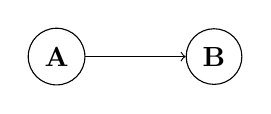
\begin{tikzpicture}[node distance=2cm]
        \node[circle,draw] at (0,0) (A) {\bf A};
        \node[circle,draw,right of=A] (B) {\bf B};
        \draw[->] (A) -- (B);
        \end{tikzpicture}
        \caption{Direct causation}
        \label{fig:direct_causation}
    \end{subfigure}
    \hfill
    \begin{subfigure}[b]{0.3\textwidth}
        \centering
        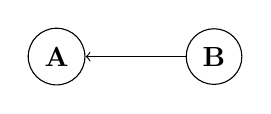
\begin{tikzpicture}[node distance=2cm]
        \node[circle,draw] at (0,0) (A) {\bf A};
        \node[circle,draw,right of=A] (B) {\bf B};
        \draw[<-] (A) -- (B);
        \end{tikzpicture}
        \caption{Reversed causation}
        \label{fig:reversed_causation}
    \end{subfigure}
    \hfill
    \begin{subfigure}[b]{0.3\textwidth}
        \centering
        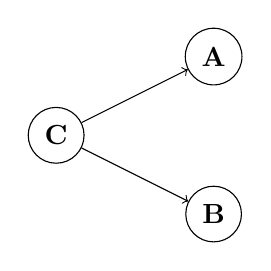
\begin{tikzpicture}[node distance=2cm]
        \node[circle,draw] at (0,0) (C) {\bf C};
        \node[circle,draw,right of=C,yshift=1cm] (A) {\bf A};
        \node[circle,draw,right of=C,yshift=-1cm] (B) {\bf B};
        \draw[->] (C) -- (A);
        \draw[->] (C) -- (B);
        \end{tikzpicture}
        \caption{Common causation}
        \label{fig:common_causation}
    \end{subfigure}
    \caption{Causal relationships.}
    \label{fig:causal_relationships}
    
\end{figure}
Determining the cause and effect from real world data is a difficult but important task. For instance proving that the emission of green house gases causes global warming is perhaps the most important task of our time. 
An example for the analysis of real ship operational data comes from a double ended ferry Uraniborg. Correlation between the thruster allocation, the utilization ratio between forward and aft thruster, was observed. Was this a direct causation or just a common causation, through a hidden variable like for instance the ocean current? 

In order to determine the causation an blinded experiment was carried out.


\begin{figure}[!htb]
    \centering
    \includegraphics[width=\textwidth]{figures/correlation.pdf}
    \caption{Fuel consumption per trip with double ended ferry Uraniborg for trips with varying aft thrust ratio}
    \label{fig:my_label}
\end{figure}



\bibliography{sample}

\end{document}